

\section{\color{red}Trær}
Et tre en et spesielt tilfelle av en rettet graf der hver node har inngrad 1 (med unntak av rota i treet). Vi ser på et eksempel:
\begin{figure}[H]
\caption{Et lite binært tre}
\label{fig:tre}
\centering
~\\
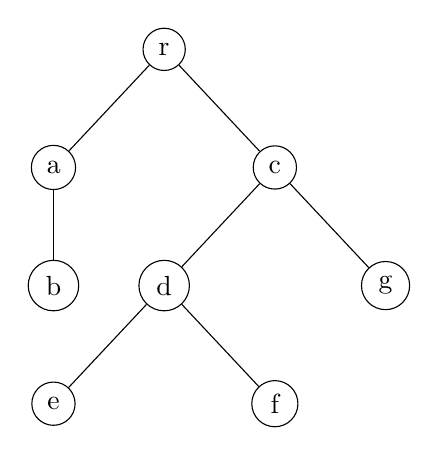
\begin{tikzpicture}[sibling distance=8em,
every node/.style = {shape=circle, draw, align=center}]

\node{r}
	child {node {a}
		child {node {b}}
	}
	child {node {c}
		child {node {d}
			child {node {e}}
			child {node {f}}
		}
		child {node {g}}
	};
\end{tikzpicture}
\end{figure}

\paragraph{Terminologi}~\\
Vi skal se litt på ord og uttrykk for trær. Gjennomgående bruker vi treet i figur \ref{fig:tre} som eksempel

I figuren blir nodene tegnet som rundinger. For å betegne relasjonen mellom nodene bruker vi ofte familierelasjoner. Vi sier at $ e $ og $ f $ er \textbf{søsken}, $ d $ er \textbf{forelder} til $ e $, og $ e $ er \textbf{barn} av $ d $. Vi kan også si at $ g $ er \textbf{onkel} til $ f $, men dette er mindre vanlig, da vi sjeldent har bruk for å snakke om \say{onkelnoder}. 

Nodene $ r, a, c $ og $ d $ kalles \textbf{indre noder}, det vil si at disse nodene har barn. Noder som ikke har noen barn kalles \textbf{løvnoder}

I figur \ref{fig:tre} er $ r $ \textbf{rotnoden}. Rota i treet er den eneste noden uten noen foreldre. Rota er derfor et naturlig startpunkt når vi skal søke eller traversere gjennom treet. 


\subsection{\color{red}Binære søketrær}
\label{bintraer}
Binære søketrær er trær med noen spesielle krav. Hver node kan ikke ha mer enn to barn, vi kaller dem ofte venstre og høyre barn. Venstre barn er alltid mindre enn noden selv, og høyre barn er alltid større enn noden. Dette gjør binære søketrær meget godt egnet for søking. 

\begin{teorem}
\label{teo:bintre}
Å sette inn, fjerne eller søke etter noder i et binært søketre har
\begin{enumerate}[i]
\item I beste fall $ O(\log n) $ tid
\item I verste fall $ O(n) $ tid
\end{enumerate}
\end{teorem}

Vi skal ikke bevise teorem \ref{teo:bintre} her\footnote{Det kan vises ved induksjon at høyden til et binært tre i beste fall er $ \log_2 n $}, men vi kan se på et eksempel som viser ytterpunktene. I figur \ref{fig:bintre} ser vi to forskjellige binære søketrær. I treet til venstre har vi et fint, balansert tre. Det er lett å se at høyden (og dermed antall operasjoner vi må gjøre for å komme til bunn i treet) er lik $ \lceil \log_2 n \rceil $ der $ n $ er antall noder i treet.

I treet til høyre har hver node kun ett barn. Vi har i praksis en lenkeliste. Hvis vi skal søke etter 4, må vi tråkke gjennom alle de andre nodene for å komme dit. 

\begin{figure}[H]
\caption{To eksempler på binære søketrær}
\label{fig:bintre}
\centering
~\\
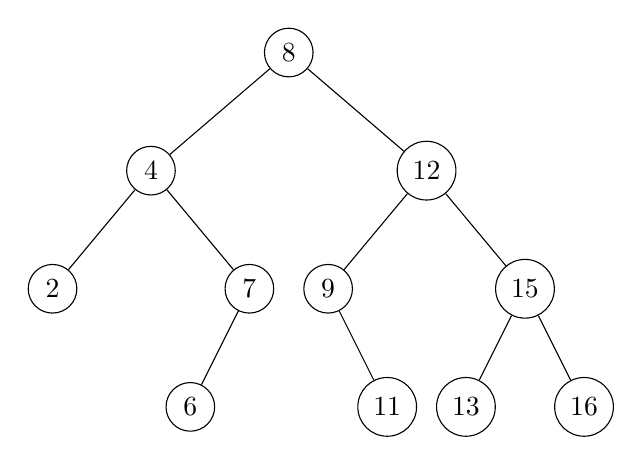
\begin{tikzpicture}[level distance=1.5cm,
  level 1/.style={sibling distance=3.5cm},
  level 2/.style={sibling distance=2.5cm},
  level 3/.style={sibling distance=1.5cm},
every node/.style = {shape=circle, draw, align=center}]

\node{8}
	child {node {4}
		child {node {2}}
		child {node {7}
			child {node {6}}
			child [missing]{}
		}
	}
	child {node {12}
		child {node {9}
			child [missing]{}
			child {node {11}}
		}
		child {node {15}
			child {node {13}}
			child {node {16}}
		}
	};
\end{tikzpicture}
$ \quad\quad $
\begin{tikzpicture}[level distance=1.5cm,sibling distance=2cm,
every node/.style = {shape=circle, draw, align=center}]

\node{1}
	child [missing] {}
	child {node {2}
		child [missing]{}
		child {node {3}
			child [missing]{}
			child {node {4}}
		}
	};
\end{tikzpicture}
\end{figure}




\paragraph{Innsetting}~\\
Når vi skal sette inn en node i et binært søketre starter vi i rota. Vi sammenligner verdien vi skal sette inn med verdien i rota. Hvis verdien vi setter inn er mindre enn rota går vil til venstre, er den større går vi til høyre. Hva som skjer ved likhet er opp til oss å bestemme, men vi må være konsekvente. Når vi kommer til en nullpeker kan vi sette denne pekeren til å peke på noden vi setter inn.

Vi kan implementere denne funksjonen rekursivt. I en ytre klasse kan vi skrive en skallfunksjon som kaller på rotas \verb|instert|-metode. Vi har en indre \verb|Node|-klasse med en rekursiv insertmetode. Den kan implementeres slik:
\javaimport{ex_bintree_insert.java}
~\\

\paragraph{Fjerning}~\\
Når vi skal fjerne en node fra et binært søketre har vi tre forskjellige situasjoner som vi må se på.

{\bfseries Noden har ingen barn} (løvnode). Denne situasjonen er ganske grei. Siden noden ikke har noen barn å forholde seg til er det bare å fjerne den fra treet.

{\bfseries Noden har ett barn}. For å fjerne en node $ a $ med ett barn kan vi ganske enkelt flytte pekeren fra foreldernoden til $ a $, til barnet til $ a $.

{\bfseries Noden har to barn}. Hvis noden vi skal fjerne har to barn
\javaimport{ex_bintree_remove.java}
~\\

\paragraph{Søking}~\\
kodeeksempel og sånt




~\\~\\
\subsection{\color{red}Rød-svarte trær}
Rødsvarte trær er binære søketrær med noen spesielle strukturkrav. Kravene er designet for å motkjempe skjevhet (som illustrert i figur \ref{fig:bintre}), og dermed forbedre kjøretid.

Vi deler nodene opp i to kategorier, røde og svarte. Vi følger noen bestemte regler på hvordan vi skal farge nodene, og fargen på nodene avgjør som vi må benytte oss av rotasjon eller ikke (se \ref{trerotasjon}). Fargen til en node er \textbf{ikke} statisk, den kan endres.

\begin{definisjon}
Et rød-svart tre er et binært søketre der hver node er
farget enten rød eller svart slik at:
\begin{enumerate}[i]
\item Roten er svart.
\item Hvis en node er rød, må barna være svarte.
\item Enhver vei fra en node til en null-peker må inneholde samme antall svarte noder.
\end{enumerate}
\end{definisjon}

\paragraph{Insetting}~\\
For å sette inn en node i rød-svarte trær kan vi bruke algoritmen i teorem \ref{teo:ins_rb}
\begin{teorem} Innsetting i rød-svarte trær. \label{teo:ins_rb}

La $ N $ være noden vi ønsker å sette inn i treet. La $ P $ være forelder, $ G $ besteforelder, og $ U $ onkel til $ N $. Følgende algoritme vil da gi en korrekt innsetting i et rød-svart tre:
\begin{enumerate}
\item Gjør innsetting som i vanlig binært søketre, der $ N $ farges rød.
\item Hvis $ N $ er rota i treet: farg $ N $ svart. 
\item Hvis $ P $ er svart: alt OK. Innsetting ferdig. 
\item Hvis $ P $ er rød og $ N $ ikke er rot:
	\begin{enumerate}
		\item Hvis $ U $ er svart:
		\begin{enumerate}
			\item Farg $ P $ svart
			\item Farg $ G $ rød
			\item Repeter fra pt. 2 med $ G $ som $ N $
		\end{enumerate}
		\item Hvis $ U $ er rød:
		\begin{enumerate}
			\item $ N $ er venstre barn av $ P $, som er venstre barn av $ G $:\\
			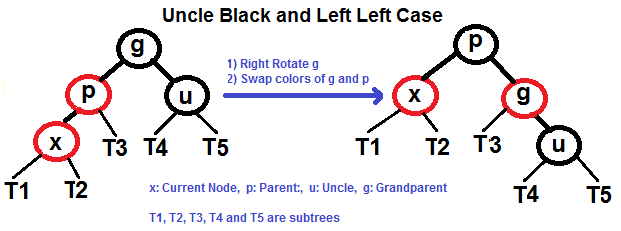
\includegraphics[width=0.65\textwidth]{rbt_ll.png}\\

			\item $ N $ er høyre barn av $ P $, som er venstre barn av $ G $:\\
			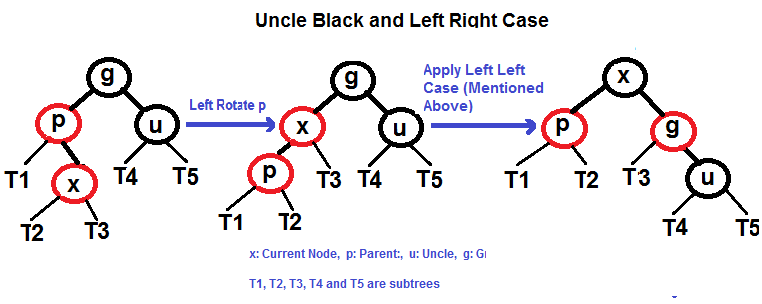
\includegraphics[width=0.65\textwidth]{rbt_lr.png}\\
			
			\item $ N $ er høyre barn av $ P $, som er høyre barn av $ G $ (speilvendt av i):\\
			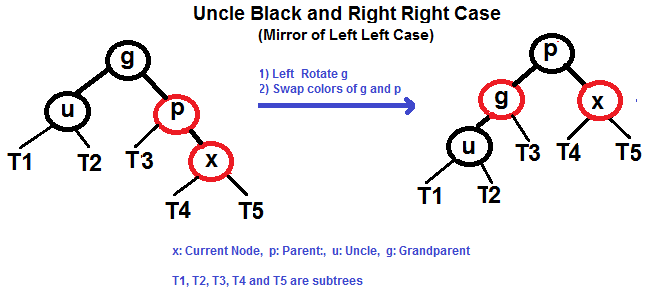
\includegraphics[width=0.65\textwidth]{rbt_rr.png}\\
			
			\item $ N $ er venstre barn av $ P $, som er høyre barn av $ G $ (speilvendt av ii):\\
			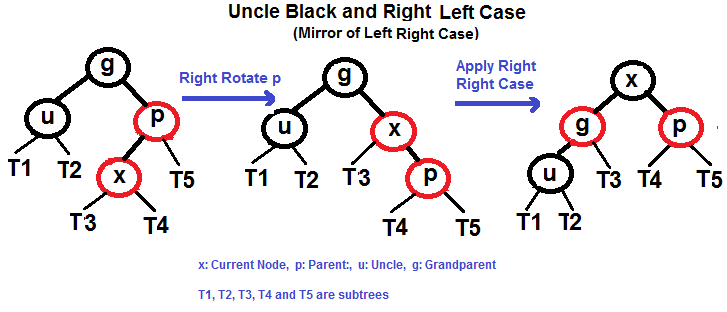
\includegraphics[width=0.65\textwidth]{rbt_rl.png}\\
			
		\end{enumerate}
	\end{enumerate}
\end{enumerate}
\end{teorem}





\subsection{\color{red}B-trær}
B-trær er konstruert for å effektivisere antall disklesninger, og gir mening å bruke hvis vi har et tre som er så stort at det må lagres på gammeldagse spinnedisker, og ikke i RAM. Vi lagrer dataene i blokker, og leser en og en blokk av gangen. Alle dataene er lagret i løvnodene, mens de indre nodene brukes for søking. B-trær er ikke binære, dvs at de kan ha flere enn 2 barn. 

\begin{definisjon} La $ M $ angi antall mulige nøkler i hver indre node, og $ L $ angi maksimalt antall dataelementer i hver løvnode. B-trær er søketrær der følgende kriterier er oppfylt:
\begin{enumerate}[i]
\item Alle dataene er lagret i løvnodene
\item Interne noder lagrer inntil $ M-1 $ nøkler for søking: nøkkel $ i $ angir den minste verdien i subtre $ i+1 $.
\item Roten er enten en løvnode, eller har mellom 2 og $ M $ barn. 
\item Alle andre indre noder har mellom $ \lceil M/2\rceil $ og $ M $ barn. 
\item Alle løvnoder har samme dybde.
\item Alle løvnoder har mellom $ \lceil L/2\rceil $ og $ L $ dataelementer
\end{enumerate}
\end{definisjon}


\paragraph{Innsetting}~\\







\subsection{\color{red}Rotasjon}
\label{trerotasjon}
\subsubsection{\color{red}Zig}

\subsubsection{\color{red}Zig-zag}
